\section{Teorema da superposição. Transformação de fontes}

\frame{
	\frametitle{Teorema da superposição}
	\begin{block}{Introdução}
		Como visto anteriormente, se um circuito tiver \textbf{duas ou mais fontes de tensão ou corrente}, uma maneira de determinar o valor de uma variável específica (tensão ou corrente) é usar a \textbf{análise nodal ou a de malhas}.
		\begin{itemize}
			\item Uma outra forma é determinar a \textbf{contribuição de cada fonte independente} à variável e então somá-las. Este método é conhecido como \textbf{superposição}.
		\end{itemize}
	\end{block}
}

\frame{
	\frametitle{Teorema da superposição}
	\begin{block}{Definição}
		O princípio da superposição afirma que a tensão (ou a corrente) em um circuito linear é a \textbf{soma algébrica das tensões (ou das correntes)} naquele elemento em virtude da atuação isolada de cada uma das fontes.
	\end{block}
}

\frame{
	\frametitle{Teorema da superposição}
	\begin{block}{Importante}
		\begin{itemize}
			\item Consideramos uma fonte independente \textbf{por vez} enquanto todas as \textbf{demais fontes estão desligadas}.
			      \begin{itemize}
				      \item\normalsize Substitua cada \textbf{fonte de tensão} por \SI{0}{\volt} (ou um \textbf{curto-circuito}).
				      \item\normalsize Substitua cada \textbf{fonte de corrente} por 0 A (ou um \textbf{circuito aberto}).
			      \end{itemize}
		\end{itemize}
	\end{block}
}

\frame{
	\frametitle{Teorema da superposição}
	\begin{block}{Etapas}
		\textbf{Na análise por superposição estamos interessados em encontrar a contribuição individual de cada fonte de tensão ou corrente, e depois somá-las}. Dado um circuito com $n$ fontes, faça: \\
		\begin{enumerate}
			\item \textbf{Desative todas as fontes}, exceto uma delas. Encontre a saída (tensão ou corrente) em razão dessa fonte ativa utilizando uma das técnicas vistas anteriormente.
			      \saveenumerate
		\end{enumerate}
	\end{block}
}

\frame{
	\frametitle{Teorema da superposição}
	\begin{block}{Etapas}
		\textbf{Na análise por superposição estamos interessados em encontrar a contribuição individual de cada fonte de tensão ou corrente, e depois somá-las}. Dado um circuito com $n$ fontes, faça: \\
		\begin{enumerate}
			\restoreenumerate
			\item Repita a etapa 1 para cada uma das \textbf{demais fontes}.
			      \saveenumerate
		\end{enumerate}
	\end{block}
}

\frame{
	\frametitle{Teorema da superposição}
	\begin{block}{Etapas}
		\textbf{Na análise por superposição estamos interessados em encontrar a contribuição individual de cada fonte de tensão ou corrente, e depois somá-las}. Dado um circuito com $n$ fontes, faça: \\
		\begin{enumerate}
			\restoreenumerate
			\item Encontre a \textbf{contribuição total} somando algebricamente todas as contribuições em razão das fontes independentes.
		\end{enumerate}
	\end{block}
}

\frame{
	\frametitle{Teorema da superposição - Exemplo $\#01$}
	\centerline{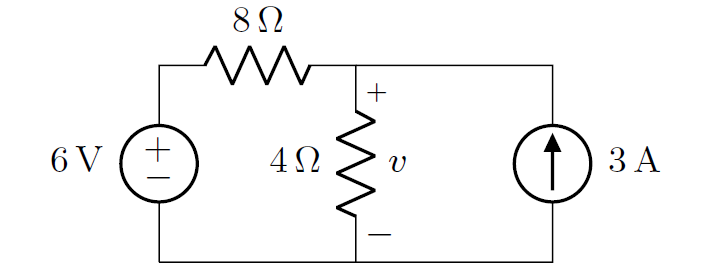
\includegraphics[width=0.5\linewidth]{Figuras/Ch04/fig1.PNG}}
	\begin{block}{Resolução - \textbf{Circuito 1}}
		\centerline{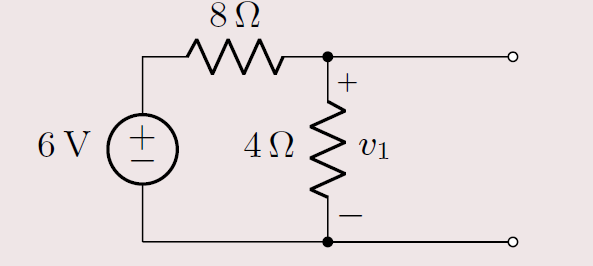
\includegraphics[width=0.45\linewidth]{Figuras/Ch04/fig2.PNG}}

		Utilizando \textbf{divisor de tensão}, temos que $v_1 = 6 \cdot \dfrac{4}{4+8} = \dfrac{24}{12} = \SI{2}{\volt}$
	\end{block}
}

\frame{
	\frametitle{Teorema da superposição - Exemplo $\#01$}
	\centerline{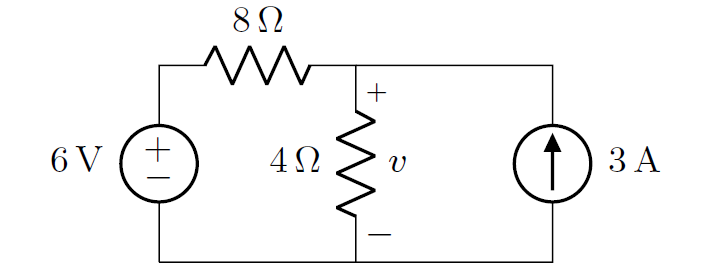
\includegraphics[width=0.5\linewidth]{Figuras/Ch04/fig1.PNG}}

	\begin{block}{Resolução - \textbf{Circuito 2}}
		\centerline{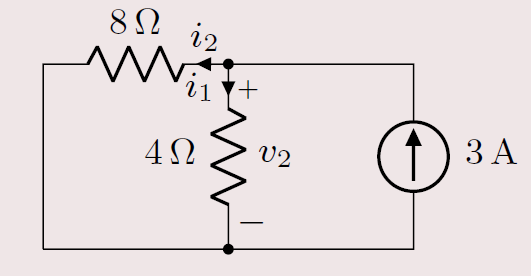
\includegraphics[width=0.45\linewidth]{Figuras/Ch04/fig3.PNG}}

		Utilizando \textbf{divisor de corrente}, temos que $i_1 = 3 \cdot \dfrac{8}{4+8} = \dfrac{24}{12} = \SI{2}{\ampere} \therefore v_2 = 4 \cdot 2 = \SI{8}{\volt}$
	\end{block}
}

\frame{
	\frametitle{Teorema da superposição - Exemplo $\#01$}
	\centerline{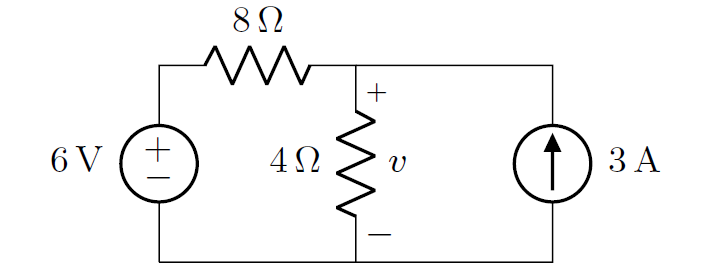
\includegraphics[width=0.5\linewidth]{Figuras/Ch04/fig1.PNG}}
	\begin{block}{Resolução}
		Como $v_1 = \SI{2}{\volt} $ e $v_2 = \SI{8}{\volt}$, temos que pelo teorema da superposição $v = v_1 + v_2 = 2 + 8 = \SI{10}{\volt}$
	\end{block}
}

\frame{
	\frametitle{Teorema da superposição - Exemplo $\#02$}
	\centerline{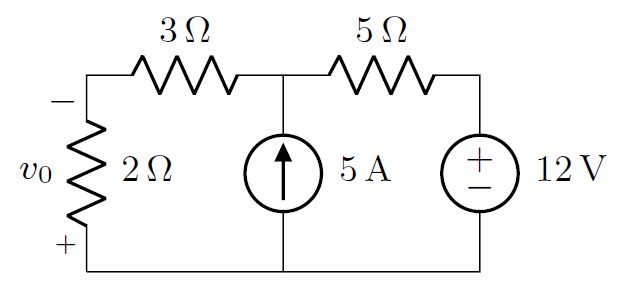
\includegraphics[width=0.5\linewidth]{Figuras/Ch04/fig4.PNG}}
	\begin{block}{Resolução - \textbf{Circuito 1}}
		\centerline{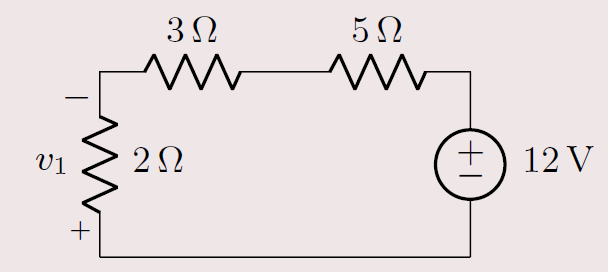
\includegraphics[width=0.45\linewidth]{Figuras/Ch04/fig5.PNG}}

		Utilizando \textbf{divisor de tensão}, temos que $v_1 = 12 \cdot \dfrac{2}{2+3+5} = \dfrac{24}{10} = \SI{2.4}{\volt}$
	\end{block}
}

\frame{
	\frametitle{Teorema da superposição - Exemplo $\#02$}
	\centerline{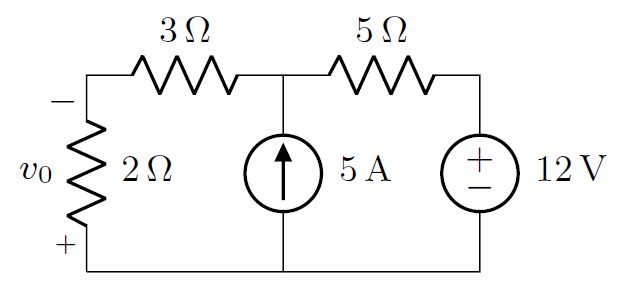
\includegraphics[width=0.5\linewidth]{Figuras/Ch04/fig4.PNG}}

	\begin{block}{Resolução - \textbf{Circuito 2}}
		\centerline{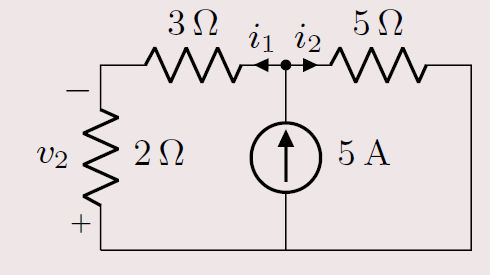
\includegraphics[width=0.4\linewidth]{Figuras/Ch04/fig6.PNG}}

		Utilizando \textbf{divisor de corrente}, temos que $i_1 = 5 \cdot \dfrac{2+3}{2+3+5} = \SI{2.5}{\ampere} \therefore v_2 = 2 \cdot \num{2.5} = \SI{5}{\volt}$
	\end{block}
}

\frame{
	\frametitle{Teorema da superposição - Exemplo $\#02$}
	\centerline{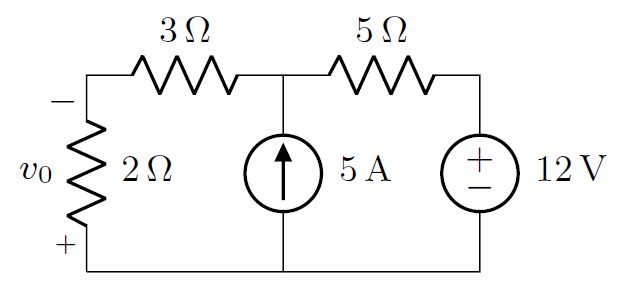
\includegraphics[width=0.5\linewidth]{Figuras/Ch04/fig4.PNG}}

	\begin{block}{Resolução}
		Como $v_1 = \SI{2.4}{\volt} $ e $v_2 = \SI{5}{\volt} $, temos que pelo teorema da superposição $v_0 = v_1 + v_2 = \num{2.4} + 5 = \SI{7.4}{\volt}$
	\end{block}
}

\frame{
	\frametitle{Transformação de fontes}
	\begin{block}{Introdução}
		A transformação de fontes é outra ferramenta que ajuda a simplificar os circuitos. É conveniente, em análise de circuitos, sermos capazes de substituir uma \textbf{fonte de tensão em série com um resistor} por uma \textbf{fonte de corrente em paralelo com um resistor}, ou vice-versa. Qualquer uma dessas situações é conhecida como \textbf{transformação de fontes}.

		\vspace{0.5cm}
		\centerline{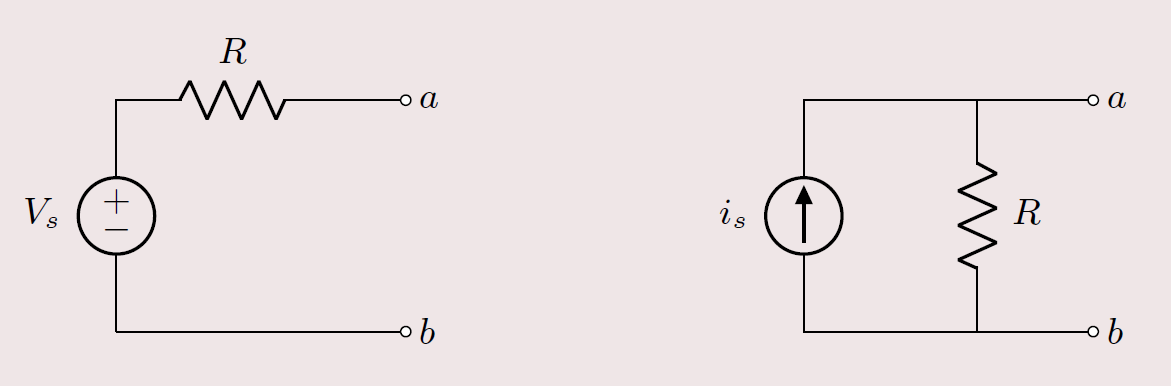
\includegraphics[width=0.9\linewidth]{Figuras/Ch04/fig7.PNG}}
	\end{block}
}

\frame{
	\frametitle{Transformação de fontes}
	\begin{block}{Definição}
		Os dois circuitos são \textbf{equivalentes}, desde que tenham a mesma relação tensão-corrente nos terminais $a-b$.
		\begin{itemize}
			\item Se as fontes forem desativadas, a resistência equivalente nos terminais $a-b$ em ambos os circuitos será $R$.
			\item Da mesma forma, quando os terminais $a-b$ forem curto-circuitados, a corrente de curto-circuito fluindo de $a$ para $b$ é $i_{sc}=V_s/R$ no circuito da esquerda, e $i_{sc} = i_s$ para o circuito da direita.
		\end{itemize}
		\vspace{0.5cm}
		Portanto, a transformação de fontes requer que \\
		$$\boxed{V_s = i_s \cdot R} \text{ ou } \boxed{i_s = \dfrac{V_s}{R}}$$
	\end{block}
}

\frame{
	\frametitle{Transformação de fontes}
	\begin{block}{Atenção}
		Devemos observar o detalhe que a fonte de corrente deve ter a seta sempre saindo do polo positivo da fonte de tensão, e vice-versa.
	\end{block}
}

\frame{
	\frametitle{Transformação de fontes - Exemplo}
	\centerline{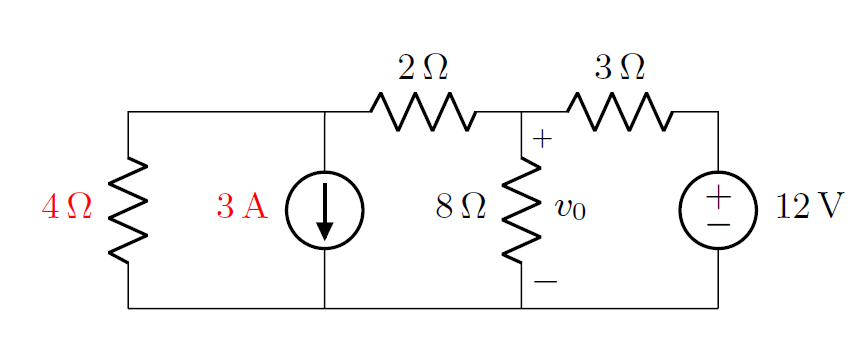
\includegraphics[width=0.8\linewidth]{Figuras/Ch04/fig8.PNG}}

	\begin{block}{Resolução - \textbf{Transformação de fontes}}
		\centerline{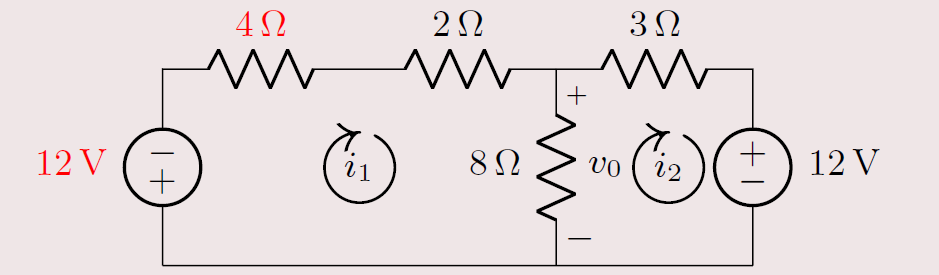
\includegraphics[width=0.8\linewidth]{Figuras/Ch04/fig9.PNG}}
	\end{block}
}

\frame{
	\frametitle{Transformação de fontes - Exemplo}
	\begin{block}{Resolução - \textbf{Análise de malhas}}
		\centerline{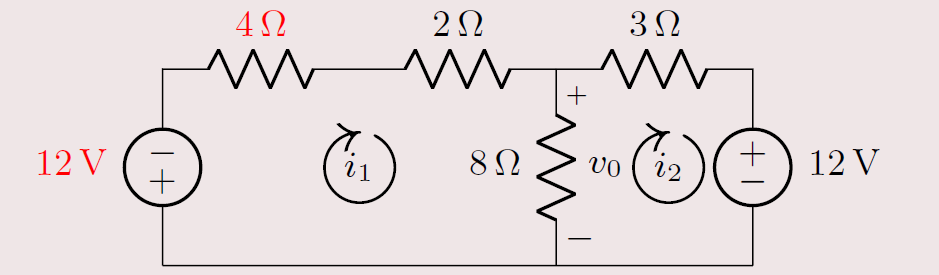
\includegraphics[width=0.8\linewidth]{Figuras/Ch04/fig9.PNG}}
		\vspace{0.2cm}

		\textbf{Malha 1}: $-12 + 6 \cdot i_1 + 8 \cdot (i_1 - i_2) = 0 \implies 7 \cdot i_1 - 4 \cdot i_2 = 6$

		\vspace{0.2cm}

		\textbf{Malha 2}: $8 \cdot (i_2 - i_1) + 3 \cdot i_2 - 12 = 0 \implies -8 \cdot i_1 + 11 \cdot i_2 = 12$

		\vspace{0.2cm}

		Resolvendo pela Regra de Cramer, temos $\boxed{i_1 = \SI{2.53}{\ampere}}$ e  $\boxed{i_2 = \SI{2.93}{\ampere}}$ \\

		\vspace{0.2cm}

		Então, $v_0 = 8 \cdot (\num{2,93} - \num{2,53}) = \SI{3.2}{\volt} $
	\end{block}
}

\frame{
	\frametitle{Associação de fontes}
	\begin{block}{Fonte de tensão em série}
		A associação em série de fontes de tensão permite \textbf{aumentar a diferença de potencial} disponibilizada para efeitos de alimentação de um circuito. Um \textbf{exemplo} da associação em série de fontes é a utilização de \textbf{múltiplas pilhas} para alimentar aparelhos eletrodomésticos, lanternas, rádios portáteis, etc. Com efeito, é comum associarem-se em série quatro pilhas de \SI{1.5}{\volt} para definir uma fonte de alimentação de \SI{6}{\volt}.
	\end{block}
}

\frame{
	\frametitle{Associação de fontes}
	\begin{block}{Fonte de tensão em série}
		A tensão disponível aos terminais de uma associação em série de fontes de tensão é dada pela \textbf{soma das tensões parciais}.
		\begin{itemize}
			\item Polaridades concordantes adicionam-se.
			\item Polaridades discordantes subtraem-se.
		\end{itemize}

		\vspace{0.5cm}

		\centerline{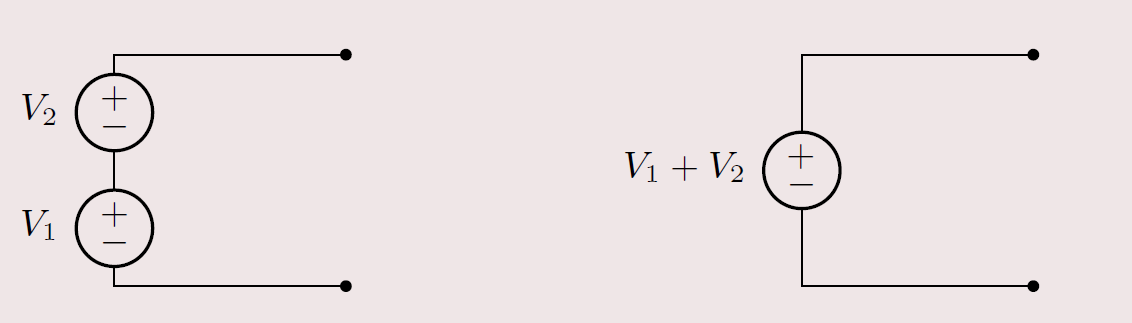
\includegraphics[width=0.9\linewidth]{Figuras/Ch04/fig10.PNG}}
	\end{block}
}

\frame{
	\frametitle{Associação de fontes}
	\begin{block}{Fonte de tensão em série}
		A tensão disponível aos terminais de uma associação em série de fontes de tensão é dada pela \textbf{soma das tensões parciais}.
		\begin{itemize}
			\item Polaridades concordantes adicionam-se.
			\item Polaridades discordantes subtraem-se.
		\end{itemize}

		\vspace{0.5cm}

		\centerline{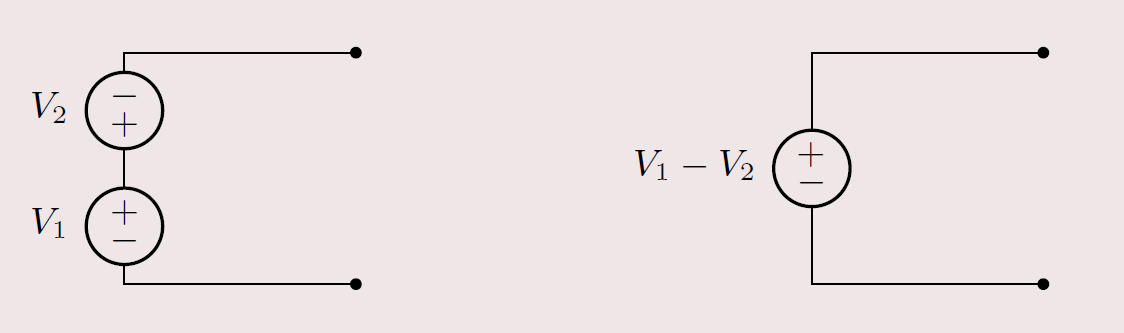
\includegraphics[width=0.9\linewidth]{Figuras/Ch04/fig11.PNG}}
	\end{block}
}

\frame{
	\frametitle{Associação de fontes}
	\begin{block}{Fonte de tensão em paralelo}
		Esta associação resultará em uma \textbf{mesma tensão} mas haverá um \textbf{somatório das correntes}. Quando há fontes de tensão diferentes, haverá um desequilibro e uma fonte começara a \textbf{drenar energia ao invés de fornecer}. Por este mesmo motivo, esta ligação para fontes de tensão apesar de possível é \textbf{muito pouco usual}.
	\end{block}
}

\frame{
	\frametitle{Associação de fontes}
	\begin{block}{Fonte de corrente em série}
		A associação de fontes de corrente em série \textbf{só} é permitida quando
		as duas fontes de corrente são \textbf{idênticas}, caso contrário,
		tem-se uma situação imprevisível (\textbf{não verificação da LKC}) e, portanto, não usual. \\
		\vspace{0.5cm}
		\centerline{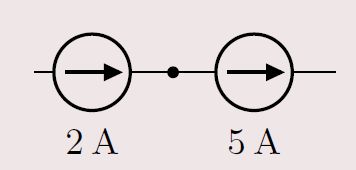
\includegraphics[width=0.3\linewidth]{Figuras/Ch04/fig12.PNG}}
	\end{block}
}

\frame{
	\frametitle{Associação de fontes}
	\begin{block}{Fonte de corrente em paralelo}
		A corrente colocada aos terminais de uma associação em paralelo é dada pela \textbf{soma das correntes parciais}, que naturalmente deve ter em conta as polaridades respectivas.
		\begin{itemize}
			\item Polaridades concordantes adicionam-se.
			\item Polaridades discordantes subtraem-se.
		\end{itemize}

		\vspace{0.5cm}

		\centerline{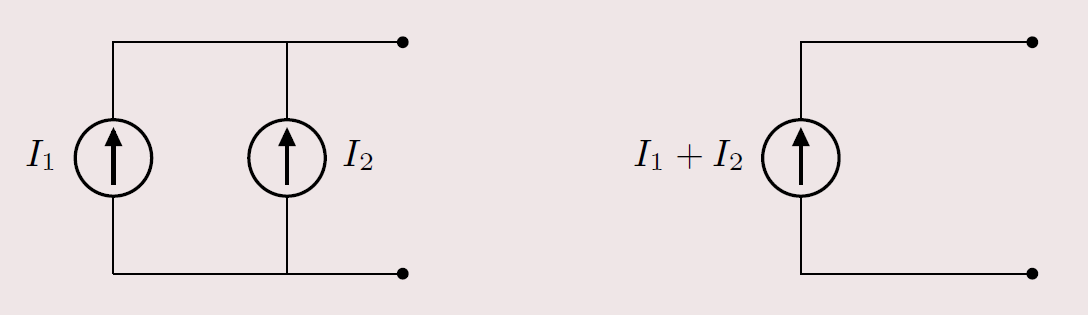
\includegraphics[width=0.9\linewidth]{Figuras/Ch04/fig13.PNG}}
	\end{block}
}

\frame{
	\frametitle{Associação de fontes}
	\begin{block}{Fonte de corrente em paralelo}
		A corrente colocada aos terminais de uma associação em paralelo é dada pela \textbf{soma das correntes parciais}, que naturalmente deve ter em conta as polaridades respectivas.
		\begin{itemize}
			\item Polaridades concordantes adicionam-se.
			\item Polaridades discordantes subtraem-se.
		\end{itemize}

		\vspace{0.5cm}

		\centerline{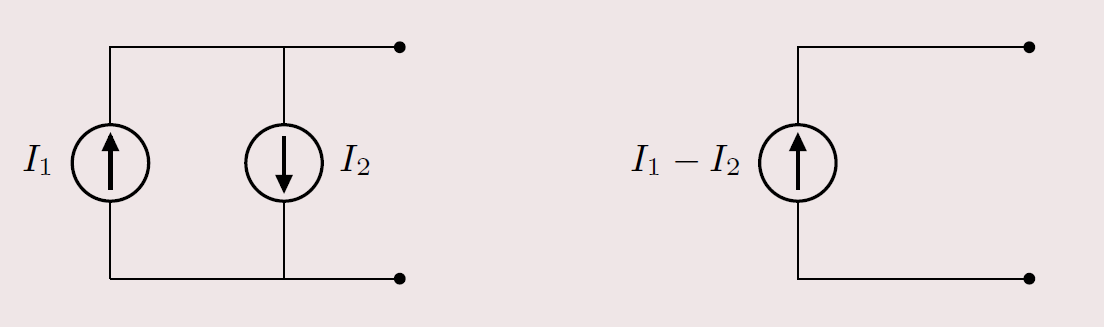
\includegraphics[width=0.9\linewidth]{Figuras/Ch04/fig14.PNG}}
	\end{block}
}

\section*{Exercícios}
\frame{
	\frametitle{Exercícios}
	\begin{block}{}
		01. Use o teorema da superposição, no circuito abaixo, para determinar $i$. \\
		\vspace{0.2cm}
		\centerline{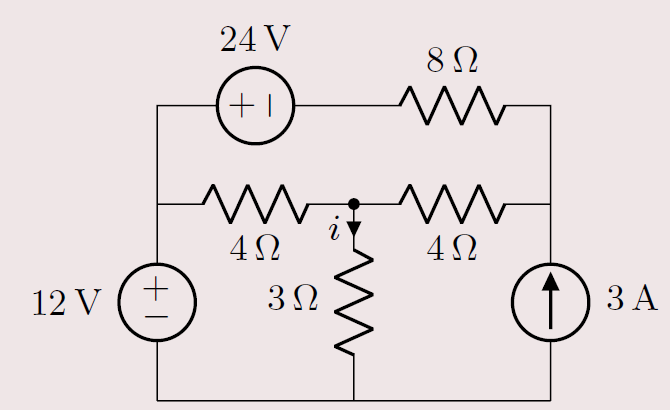
\includegraphics[width=0.6\linewidth]{Figuras/Ch04/fig15.PNG}}
	\end{block}
}

\section*{Exercícios}
\frame{
	\frametitle{Exercícios}
	\begin{block}{}
		02. Determine $i_0$ usando transformação de fontes. \\
		\vspace{0.2cm}
		\centerline{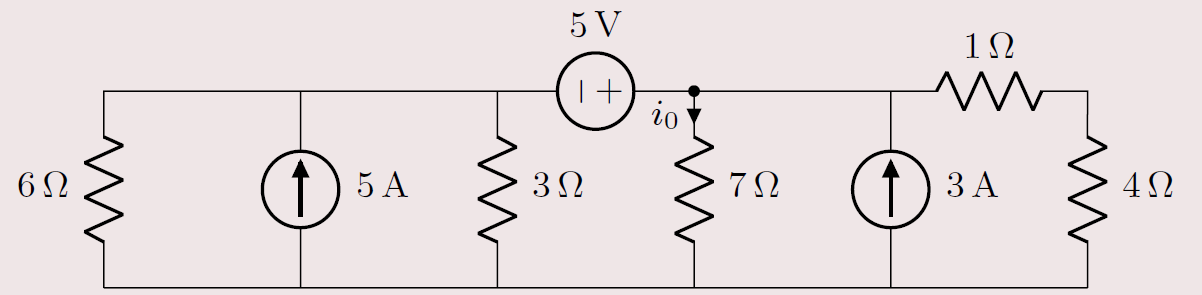
\includegraphics[width=1\linewidth]{Figuras/Ch04/fig16.PNG}}
	\end{block}
}

\section*{Referências}

\frame{
	\frametitle{Referências e Exercícios Complementares}
	\begin{itemize}
		\item ALEXANDRE, Charles K.; SADIKU, Matthew N. O. Fundamentos de Circuitos Elétricos. 5. ed. Porto Alegre: AMGH, 2013.
	\end{itemize}
	%\centering{\alert{Página 36 - \textbf{1.6.1 até 1.6.5, 1.6.17 até 1.6.19}}} \\
	\centering{\alert{Lista de exercícios 04}}
}